% !TeX spellcheck = cs_CZ
{\tikzset{external/prefix={tikz/FYZI/}}
 \tikzset{external/figure name/.add={ch39_}{}}
%=========================== Kapitola: Kinetická teorie plynů =====================================
\chapter{Kinetická teorie plynů}\label{fyz:IchapXXXIX}
\minitoc
  \section{Vlastnosti látek}\label{fyz:IchapXXXIXsecI}
  \section{Tlak plynu}\label{fyz:IchapXXXIXsecII}
  \section{Stlačitelnost záření}\label{fyz:IchapXXXIXsecIII}
  \section{Teplota a kinetická energie}\label{fyz:IchapXXXIXsecIV}
  \section{Zákon ideálního plynu}\label{fyz:IchapXXXIXsecV}
  \section{Příklady a cvičení}\label{fyz:IchapXXXIXsecVI}


    \begin{figure}[ht!] %\ref{fyz_fig242}
      \centering
      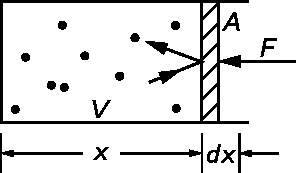
\includegraphics[width=0.5\linewidth]{fyz_fig242.pdf}
      \caption{
               (\cite[s.~525]{Feynman01})}
      \label{fyz_fig242}
    \end{figure}

    \begin{figure}[ht!] %\ref{fyz_fig243}
      \centering
      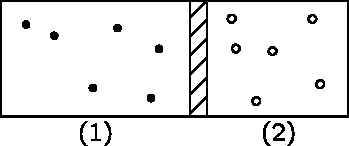
\includegraphics[width=0.5\linewidth]{fyz_fig243.pdf}
      \caption{
               (\cite[s.~530]{Feynman01})}
      \label{fyz_fig243}
    \end{figure}

    \begin{figure}[ht!] %\ref{fyz_fig244}
      \centering
      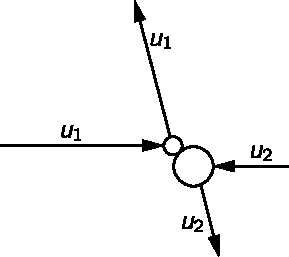
\includegraphics[width=0.5\linewidth]{fyz_fig244.pdf}
      \caption{
               (\cite[s.~531]{Feynman01})}
      \label{fyz_fig244}
    \end{figure}

    \begin{figure}[ht!] %\ref{fyz_fig245}
      \centering
      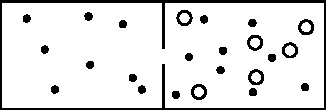
\includegraphics[width=0.5\linewidth]{fyz_fig245.pdf}
      \caption{
               (\cite[s.~533]{Feynman01})}
      \label{fyz_fig245}
    \end{figure}

} %tikzset
%---------------------------------------------------------------------------------------------------
\printbibliography[title={Seznam literatury}, heading=subbibliography]
\addcontentsline{toc}{section}{Seznam literatury}